% !TEX root = ThesisGchatzi.tex

\subsection{Experimental Evaluation}
\label{sec:evaluation}

\graphicspath{{Papers/ElsevierBigDataResearch/}}

In this section, we evaluate the proposed visualization methods. We first describe our experimental setup including the datasets that we use in the evaluation. Next, we present illustrative visualizations over real-world geolocated time series, as well as scalability results against a synthetic dataset containing 4 million geolocated time series.

\subsection{Experimental Setup}
\label{subsec:exp_setup}

All experiments were conducted on a Dell PowerEdge M910 with 256 GB RAM and 4 Intel Xeon E7-4830 CPUs, each containing 8 cores clocked at 2.13GHz. We assume that all indices fit in memory, hence parameter selection for their construction was based on this assumption. We use the water and taxi real-world datasets also used for experimental evaluation in Section~\ref{sec:exp_btsr}. To examine the scalability of our algorithms, we generated a synthetic dataset comprising 4 million geolocated time series by inflating the water consumption dataset. This was achieved by using the original time series as seeds and introducing some random variations in their location and pattern. We chose the water dataset so as to generate a more densely populated dataset (Alicante is a medium-sized city) to stress-test our summarization methods. In scalability tests, we also make use of randomly chosen subsets from this synthetic dataset. Table \ref{tab:datasets_vis} lists a summary of the main characteristics for each dataset.

\begin{table}[ht]
	\centering
	\caption{Datasets used in the experiments.}
	\begin{small}
	\centering
	\begin{tabular}{lcccccc}
	\hline
	\multirow{2}{*}{Dataset} & Area & Number of & Length $n$ of \\
	 & (km$^2$) & time series & each time series \\
	\hline
	Water & 114 & 822 & 168 \\
	Taxi & 2,500 & 417,960 & 168 \\
	Synthetic & 114 & 4,000,000 & 168 \\
	\hline
	\end{tabular}
	\end{small}
	\label{tab:datasets_vis}
\end{table}

Table~\ref{tab:parameters1} lists the range of values for the parameters used in our tests concerning both methods; default values are shown in bold.

\begin{table}[ht]
\centering
\caption{Parameters tested in the experiments.}
\begin{footnotesize}
\begin{tabular}{lc} 
\hline
{\em Parameter} &{\em Values} \\
\hline
Dataset size & 1000K, 2000K, 3000K, {\bf 4000K} \\
Map scale & 1:50000, 1:25000, 1:20000, 1:15000, 1:10000, {\bf 1:5000}, 1:500 \\
\hline
\end{tabular}
\end{footnotesize}
\label{tab:parameters1}
\end{table}

\subsection{Evaluation of Bundle Summarization}
\label{subsec:bundle_sum}

We first present a detailed evaluation of our method concerning bundle summaries. Specifically, we present two visualization examples on two real-world datasets. Then, we evaluate the scalability of our method in terms of different map scales and dataset sizes.

\subsubsection{Map Visualizations}
\label{subsubsec:bundle_sum_vis}

The visualization for the bundle summary depicts the MBTS derived for the most representative patterns of time series at the currently visible area of the map. Once our summarization method returns the results, the corresponding MBRs contained in the current view and zoom level are drawn on the map, along with the number of the geolocated time series that belong to the selected bundle. This number is depicted using circles, colored green for small numbers, yellow for larger and red for more densely populated MBRs, thus easily conveying the local intensity of this pattern. The bundles are listed on the left of the map, using confidence bands to indicate their upper and lower bounds. The average time series of each bundle is also depicted. A user can scroll this list and select the bundle of their preference. Once a bundle is selected, the contents of the map are updated accordingly with the respective MBRs and aggregates.

\begin{figure*}[ht]
 \centering
 \fbox{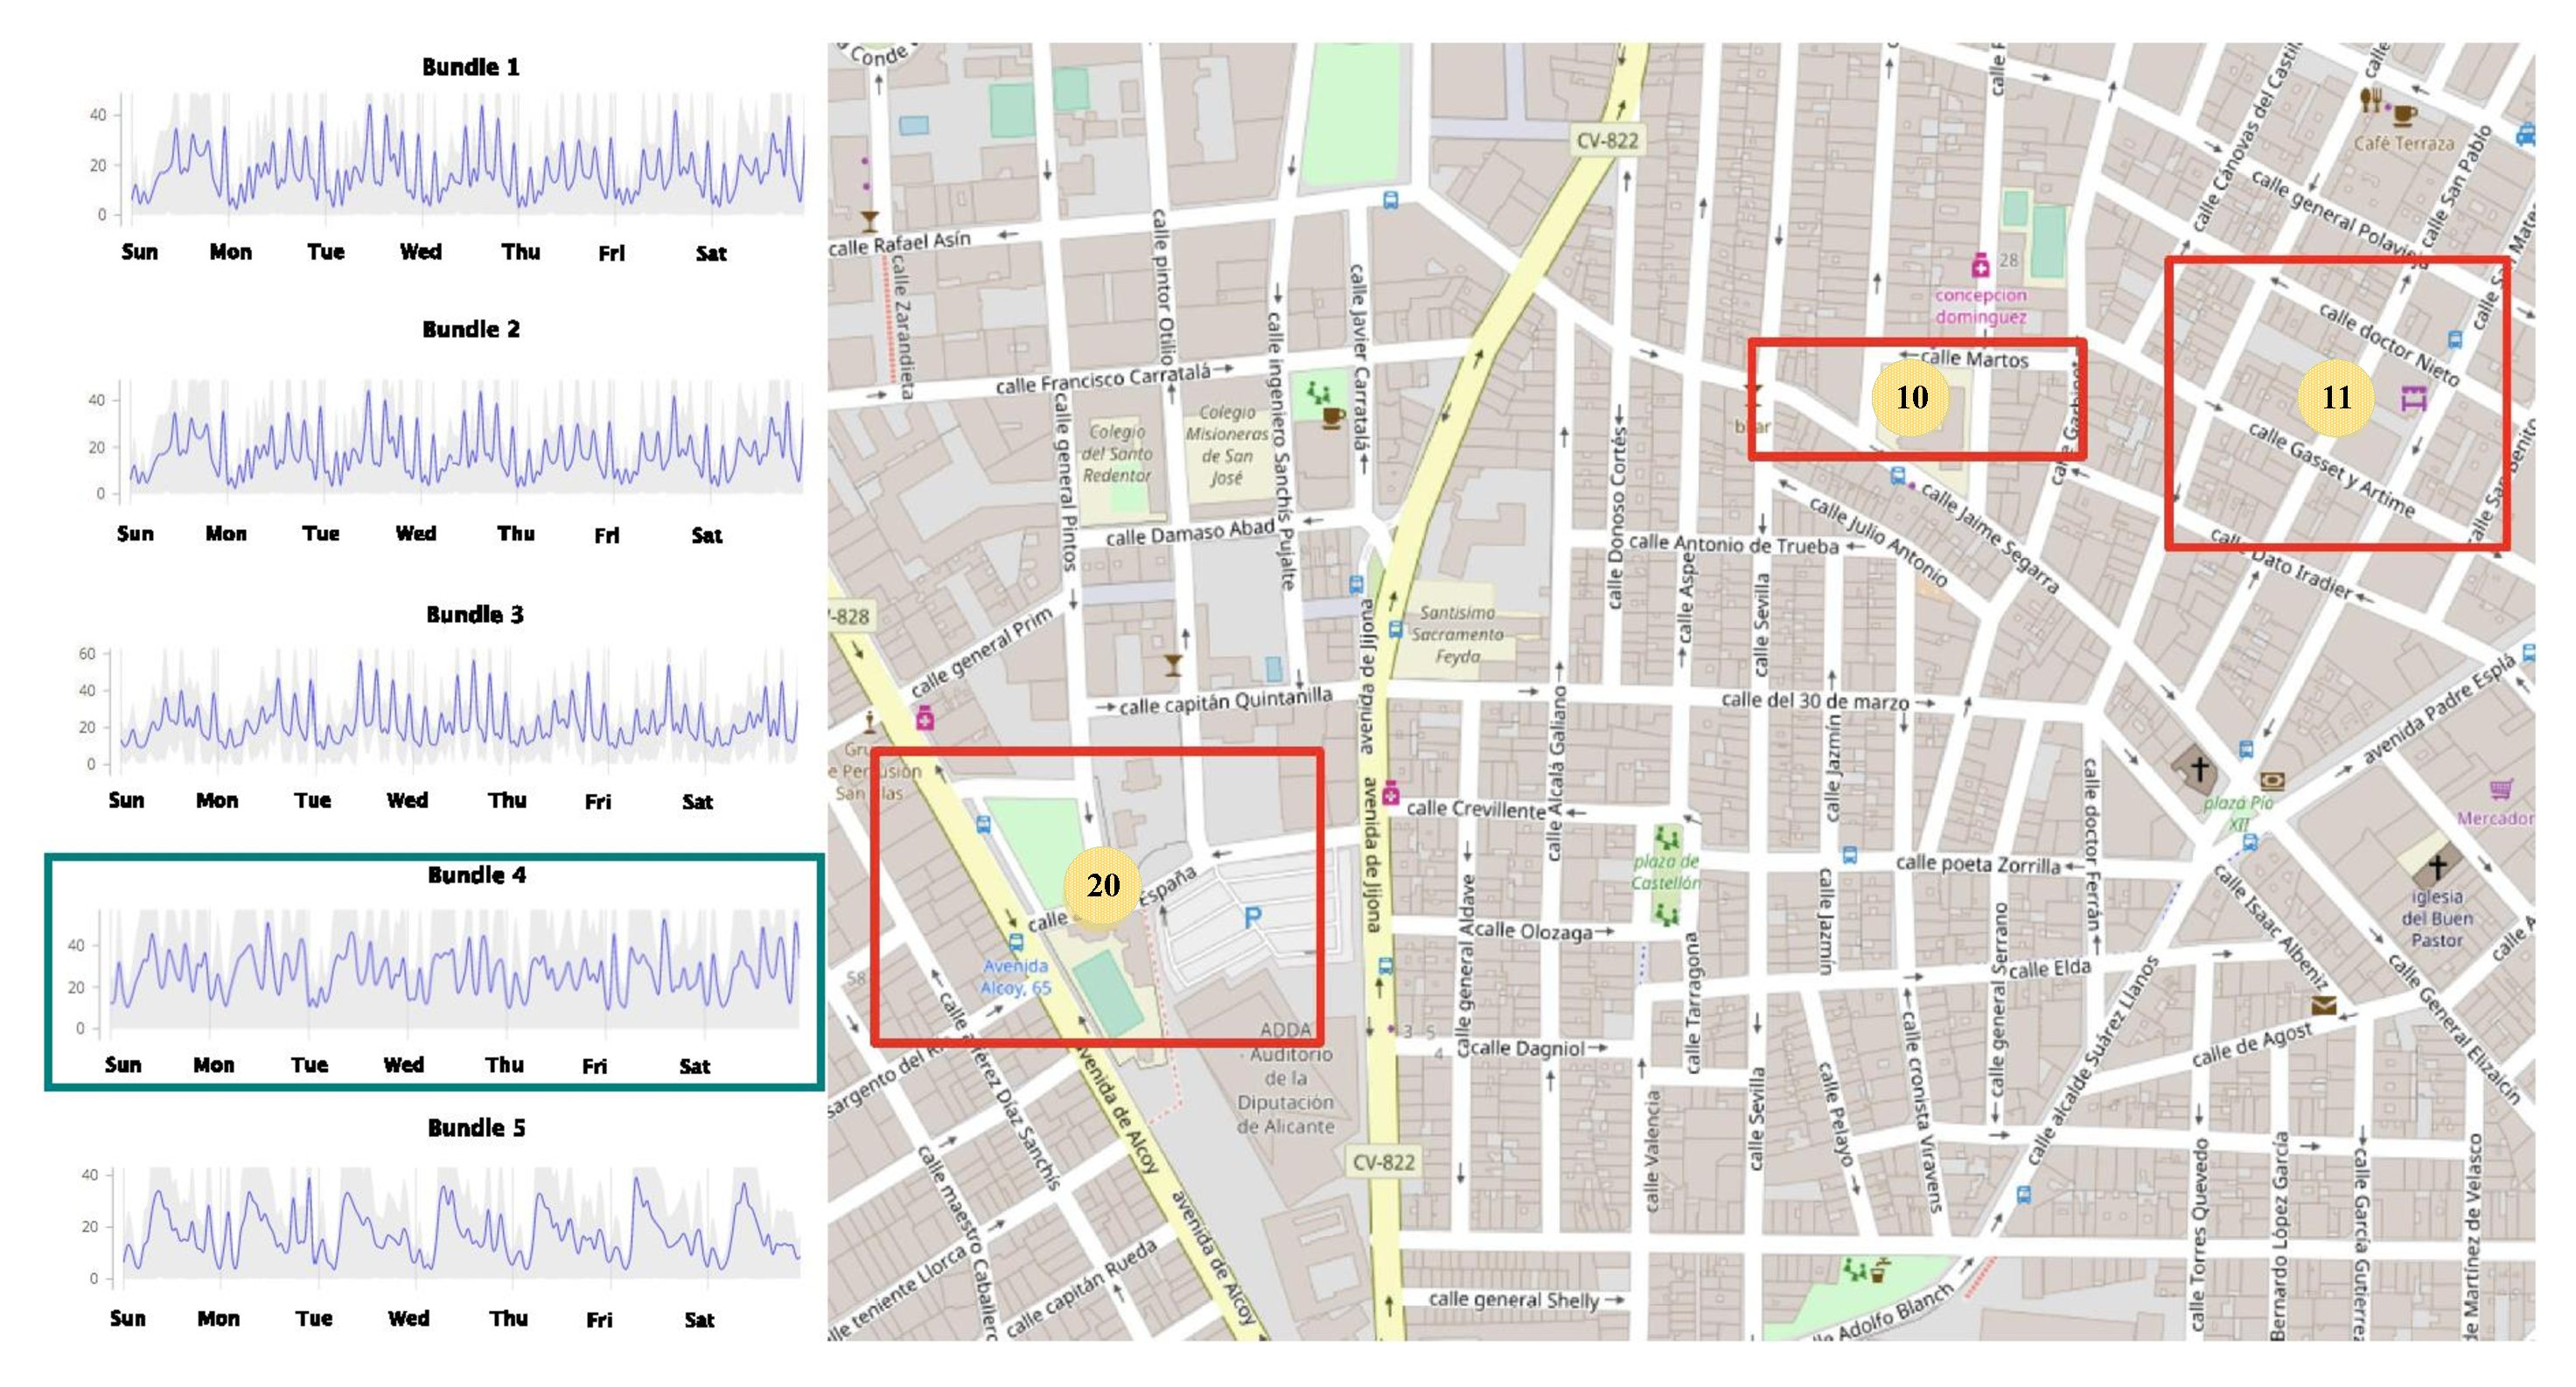
\includegraphics[width=\textwidth]{figures/alicante_btsr_explorer.pdf}}
 \caption{Visualizing water consumption patterns in the city center of Alicante (map scale 1:5000).}
 \label{fig:alicante_example}
\end{figure*}

Figure~\ref{fig:alicante_example} shows an example of the bundle summary visualization using the water dataset, for $k=5$ bundles and $l=3$ MBRs. The depicted area is in the center of Alicante, in the most densely populated zone of the city. In this example, \texttt{Bundle 4} is selected (indicated with a green colored frame) and the relevant MBRs are shown on the map (using red colored boxes). This indicates that inside each depicted MBR there exists a specific number of geolocated time series that have been clustered to the chosen bundle. As mentioned, each geolocated time series in this dataset represents hourly water consumption of a household across one week. Different consumption behaviors have been grouped together and a daily pattern for each bundle can be noticed which is due to the Circadian rhythmic way that people consume water \cite{aschoff1965circadian}. The rather large number of geolocated time series in the bundle, considering the zoom level and the extent of the MBRs, intuitively suggests that neighboring families tend to have similar water consumption behavior. 

Figure~\ref{fig:nyc_example} illustrates another example, this time using the taxi dataset in New York City, for $k=5$ bundles and $l=11$ MBRs. This dataset is significantly larger, and the zoom level selected in this example is lower (a larger geographic area is visible), hence the MBRs contain a larger number of time series. In this figure, we choose \texttt{Bundle 1}, which represents the rather quieter taxi dropoff zones in Manhattan, as the total number of dropoffs there is rarely over 60 during any hour of the week. In this example, there is also a clear daily routine in all bundles, with the dropoffs reaching a local maximum twice per day, suggesting the rush hours in New York City, when people commute to and from their work. In almost all bundles, the daily pattern is significantly different on Saturdays and Sundays, which confirms the intuition that during weekends people do not tend to commute in a routinely fashion. Overall, such visual representations of information digested from massive time series data can easily catch users' attention to important phenomena and ongoing trends, confirming the usefulness of our approach.

\begin{figure*}[ht]
 \centering
 \fbox{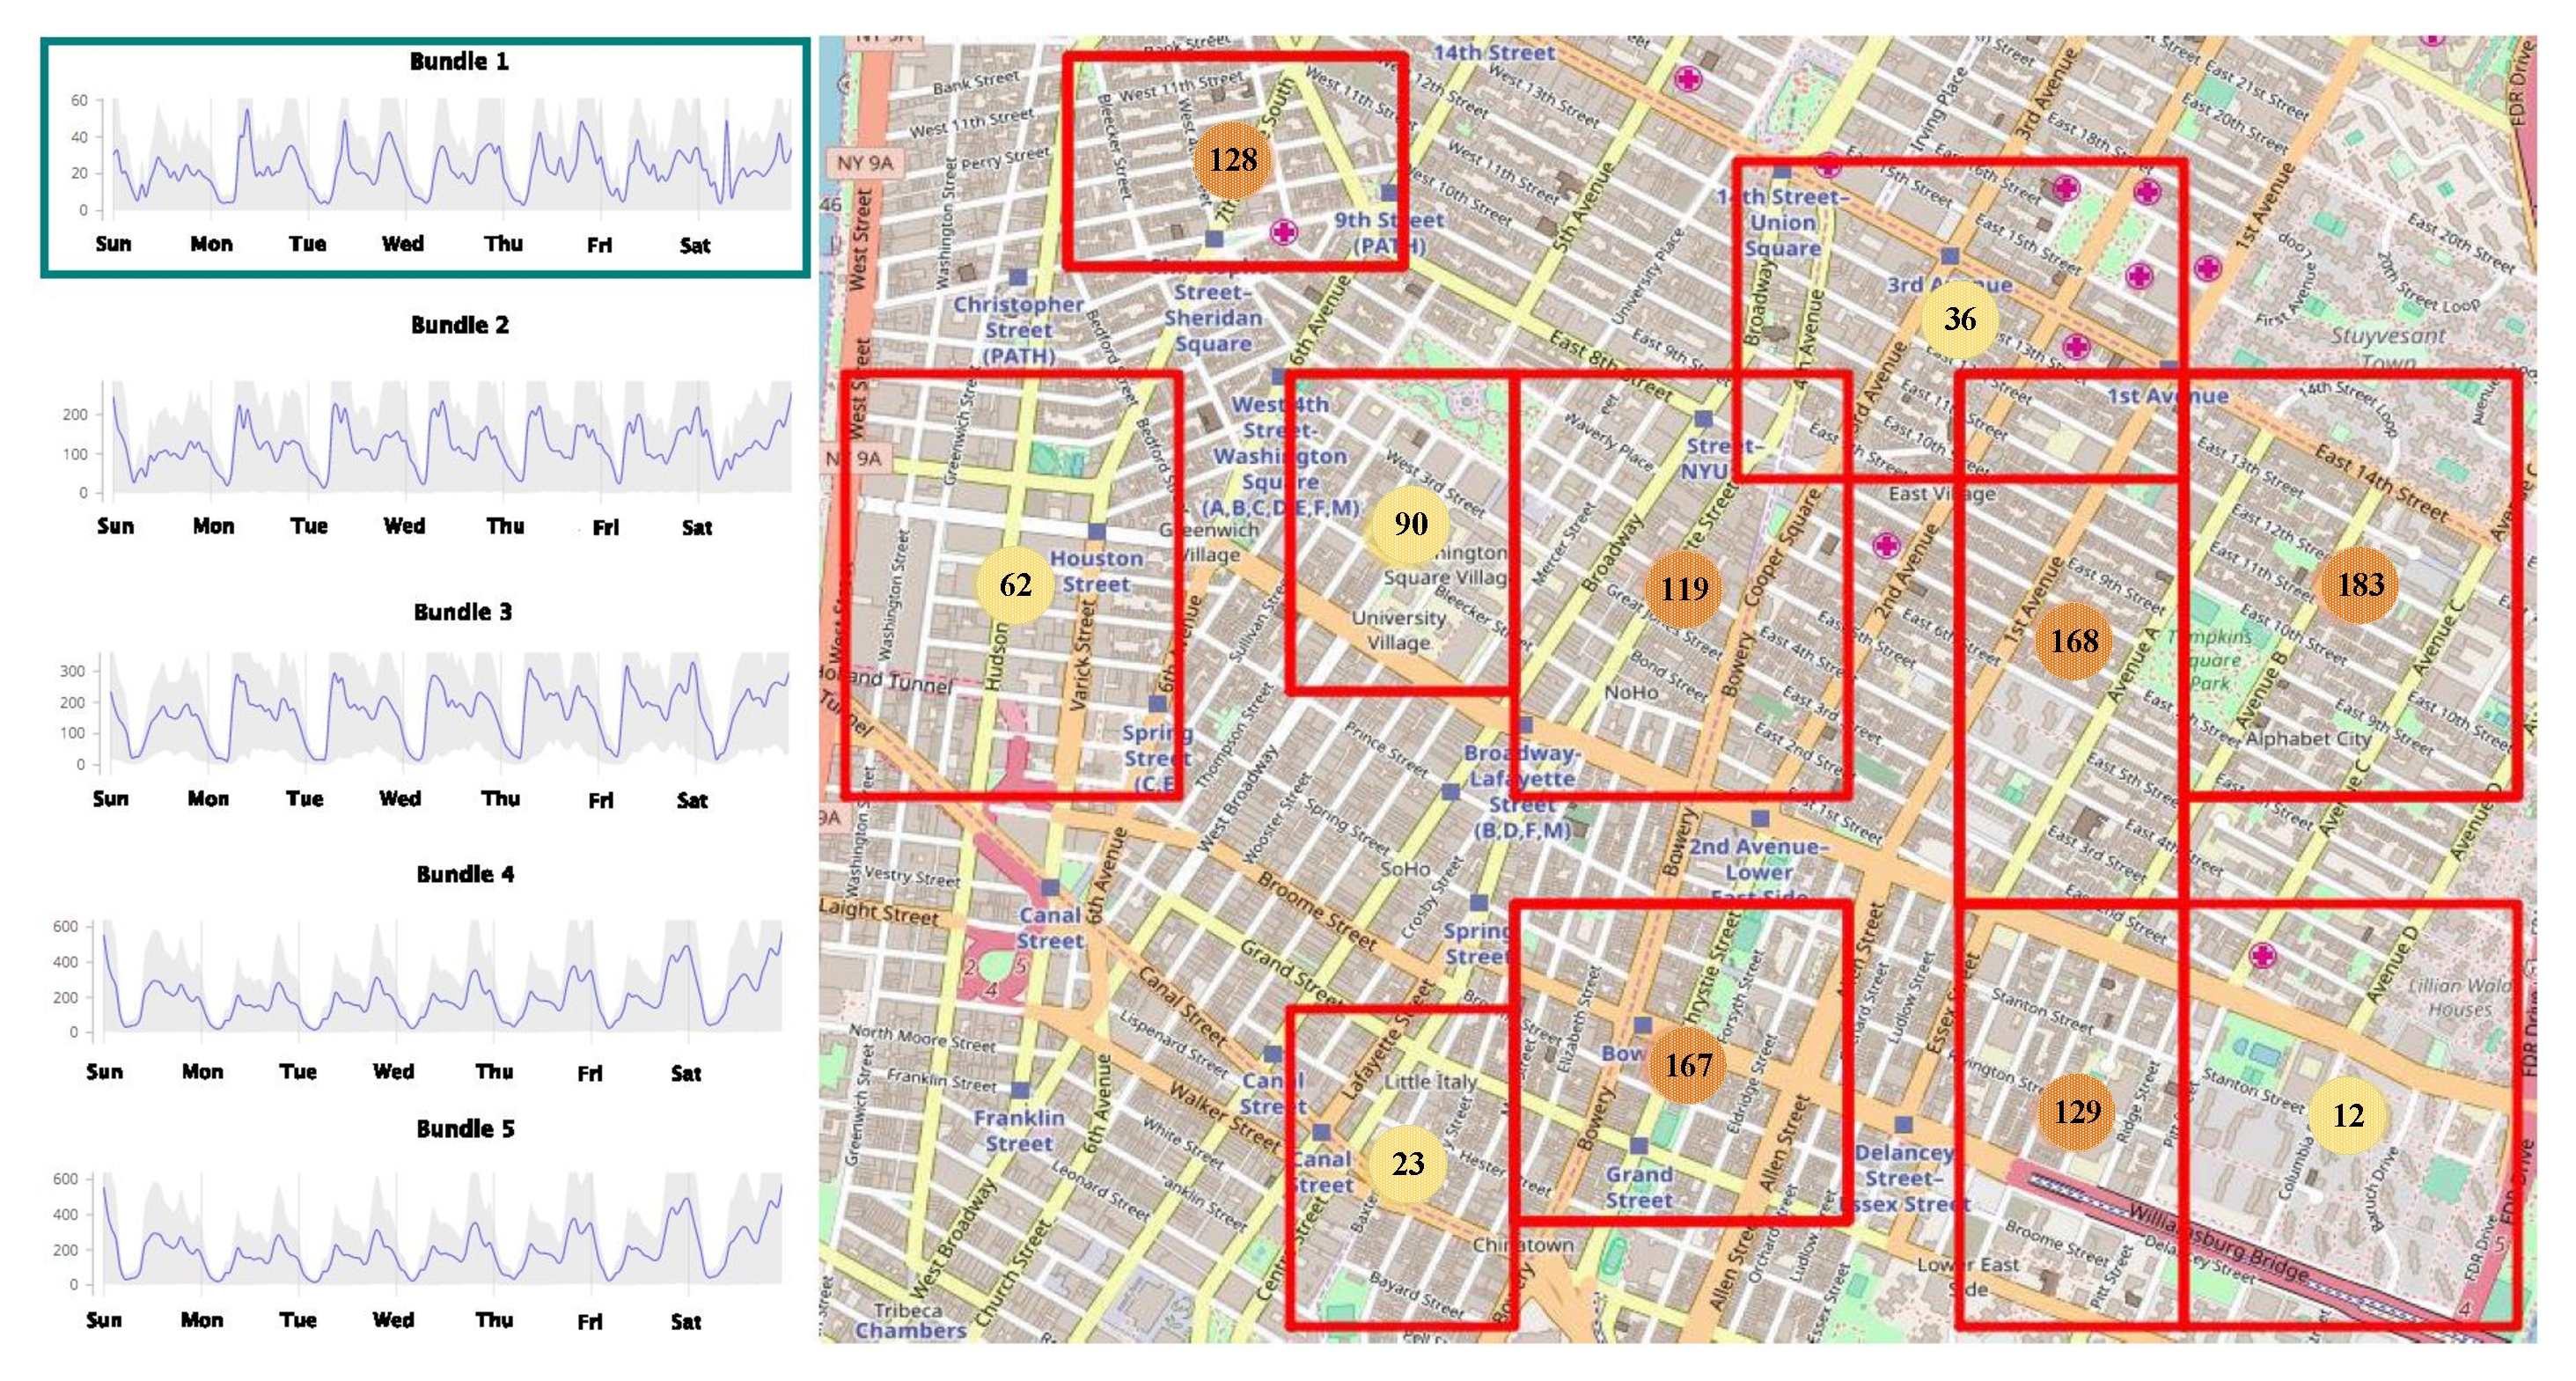
\includegraphics[width=\textwidth]{figures/nyc_btsr_explorer.pdf}}
 \caption{Visualization of taxi dropoff patterns in Manhattan, NYC (map scale 1:10000).}
 \label{fig:nyc_example}
\end{figure*}

\subsubsection{Performance Evaluation}
\label{subsubsec:bundle_sum_benchmarking}

\paragraph{Parameters.} In preliminary tests, we fine-tuned parameters used against the synthetic dataset. Conclusively, for the scalability evaluation, we built the \btsr index setting the minimum and maximum number of entries per node to $m=750$ and $M=2000$, respectively. Note that the index fits in memory, so such large parameter values do not have a negative impact on performance. For an evaluation of the \btsr index under different parameter settings, please refer to \cite{chatzig17btsr}. Regarding the number of bundles, we set $k_0 = 5$ for its leaf nodes. The number $k$ of bundles and the number $l$ of MBRs per bundle for the traversal algorithm is set to be equal to the number of bundles at the leafs, i.e., $k = l = k_0 = 5$.

\paragraph{Baseline method for Detailed Bundle Summaries.} In order to determine the trade-off between responsiveness and accuracy of our method (Section \ref{subsec:visualization}), we compare it with a baseline approach, which involves more {\em detailed summarization}. The latter utilizes the raw geolocated time series retrieved from the spatial filtering and generates the summaries by first applying $k$-means clustering on the time series domain to obtain the bundles, followed by another clustering in the spatial domain within each bundle to obtain its respective MBRs. 

\paragraph{Results.} We evaluate the performance of our approach on larger datasets in terms of response time for different zoom levels on the map using map scales, since zooming-in requires deeper traversal of the \btsr index. The comparison is performed for subsets of the synthetic dataset of different size. We measure the {\em accuracy} both in spatial and time series domains, by calculating the mean Euclidean distance of each object located within the spatial area of interest from its closest bundle and MBR, respectively. Since this is intended as an interactive application, where the summarization method is triggered as soon as the user moves the map, {\em response times} must be adequately small. In our method, this is facilitated by the fact that the search along a path stops once it encounters a node whose MBR is contained in the actual map extent (rectangle). However, for the same reason, the responsiveness is expected to come at the expense of the summaries' level of detail, since the inner nodes contain coarser information regarding the time series they contain in their sub-trees.


\begin{figure}[!ht]
 \centering
 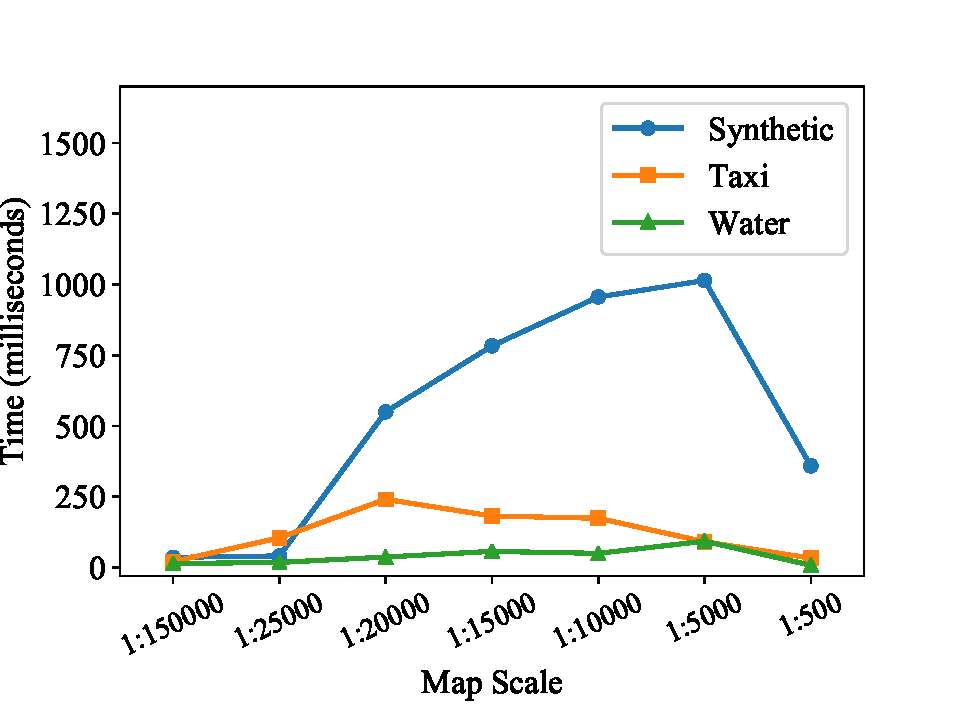
\includegraphics[width=0.75\textwidth]{figures/BTSR_zoom.pdf}
 \caption{Execution time for different map scales.}
 \label{fig:btsr_zoom}
\end{figure}


Figure~\ref{fig:btsr_zoom} depicts traversal costs for different map scales over the areas covered by the three datasets. More specifically, the water and synthetic datasets cover the area of the city of Alicante, Spain, whereas the taxi dataset the wider metropolitan area of New York City. Response time in all cases is equal or lower than one second. The synthetic dataset, due to its very high density is significantly slower than the rest, however still the results are obtained in less than a second. The response for the water dataset is almost instant due to its small size and very low density. Initially, in all cases, at the largest scale, the visible area of the map contains all the time series in the dataset, thus it only has to retrieve information from the root of the index. Then, as we zoom in, more nodes have to be visited, as the MBRs of the accessed nodes begin to overlap with the map rectangle and their children have to be retrieved. The worst case for the synthetic dataset is at scale 1:5000, which roughly corresponds to a large neighborhood of the city, where many time series are located. For the taxi dataset, the worst case is at 1:20000, which corresponds to the wider Manhattan area and then the response time gradually drops due to the lower dataset density. The number of nodes accessed in each case is proportional to the response times, ranging from one node (the root) in case of the smaller map scale (all city) up to 165 at scale of 1:5000 for the synthetic dataset, one up to 53 for the taxi dataset and one up to 15 for the water dataset. Interestingly, fewer node accesses are required in all cases at the very large scale of 1:500, since the respective small map area overlaps with fewer nodes and most of the search space is pruned. 


\begin{figure}[!ht]
 \centering
 \subfloat[Accuracy in spatial domain.]{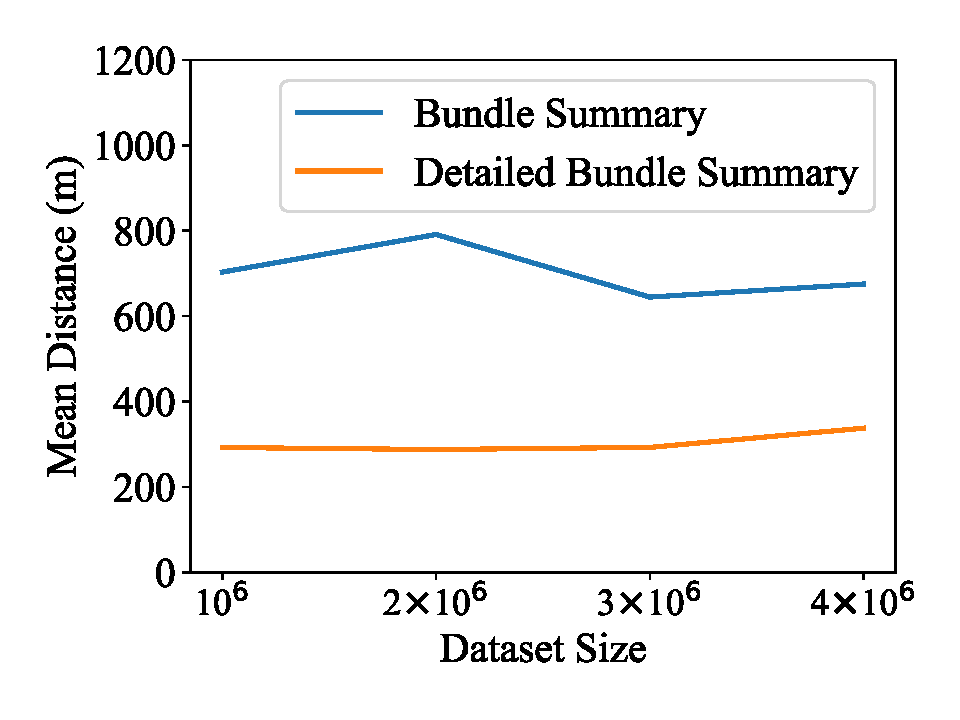
\includegraphics[width=0.30\textwidth]{figures/BTSR_error_sp.pdf}\label{subfig:btsr_error_sp}}
 \subfloat[Accuracy in time domain.]{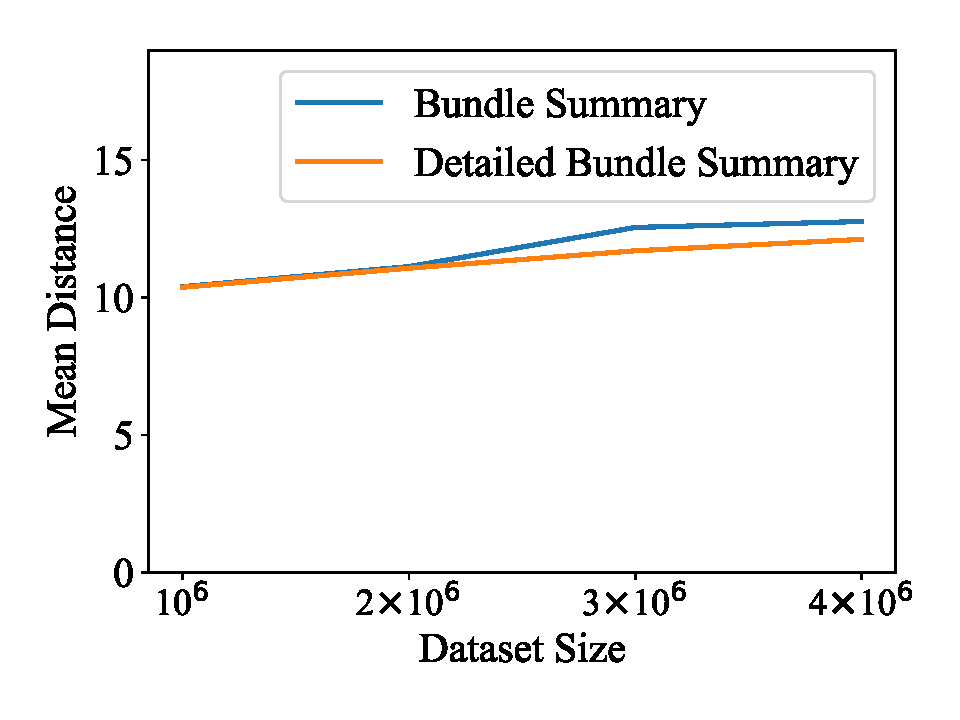
\includegraphics[width=0.30\textwidth]{figures/BTSR_error_ts.pdf}\label{subfig:btsr_error_ts}}
 \subfloat[Response time.]{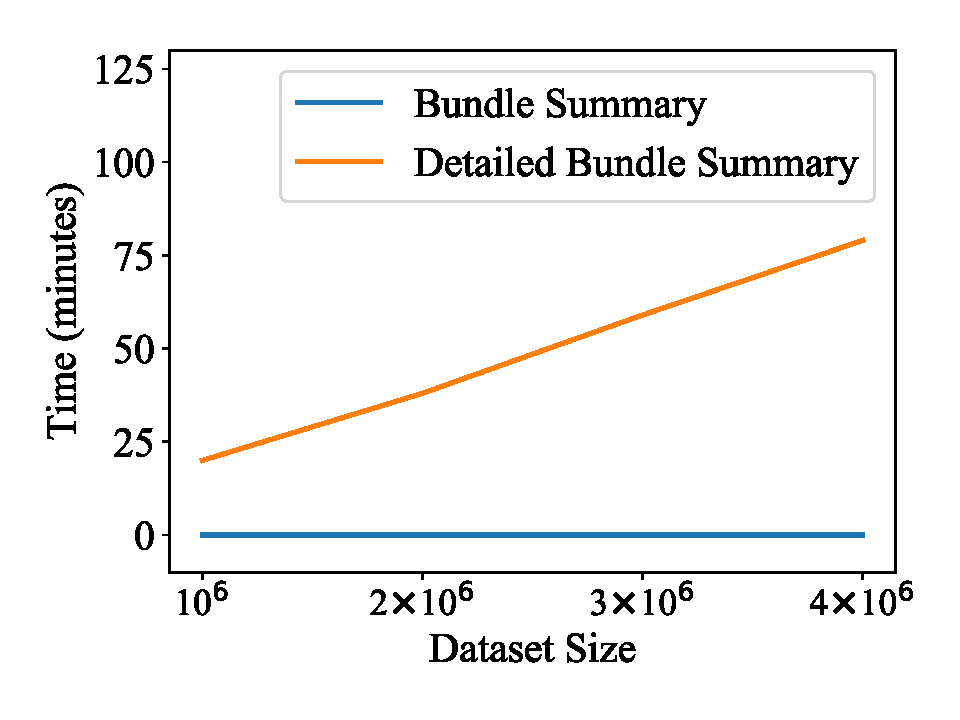
\includegraphics[width=0.30\textwidth]{figures/BTSR_time.pdf}\label{subfig:btsr_time}}\
\caption{Assessment of bundle summarization.}
\label{fig:btsr_error}
\end{figure}


Figure~\ref{fig:btsr_error} depicts the accuracy and responsiveness comparison between the bundle summarization method and its detailed version. In the spatial domain (Figure\ref{subfig:btsr_error_sp}), it is apparent that the mean Euclidean distance of the raw data from the closest MBR centers is close to two times larger for our bundle summary, indicating a loss in accuracy, as expected. The mean distance is not heavily affected by the dataset size at any case, indicating a rather stable summary quality, independent of the amount of the results. The case is quite different in the time series domain (Figure\ref{subfig:btsr_error_ts}), where the mean distance of the raw time series from the closest bundle's average time series is only slightly larger for the bundle summary --especially for smaller datasets--, indicating a rather good summary quality. There is a slight worsening trend in both cases as the size of the dataset is increased, possibly due to the tendency of the summary to be more generic as the number of results increases, with a larger number of \btsr nodes taking part in the summary calculation. However, this loss in accuracy in both domains is largely compensated in terms of execution time (Figure~\ref{subfig:btsr_time}), with the bundle summary being close to one second in all cases, while the detailed approach is linearly slowed down as the dataset size increases, requiring more than an hour to generate the summary against 4 million objects. Overall, this test confirms that our proposed method for bundle summaries can offer a really large speedup in terms of response time with tolerable concessions in accuracy, even against a heavily dense synthetic dataset where a large number of time series are contained within a small area.

\subsection{Evaluation of Tile Map Summarization}
\label{subsec:tilemap_sum}

Next, we present an evaluation of our method for obtaining tile map summaries. We first demonstrate two examples of visual exploration via summarization over two real-world geolocated time series datasets. Then, we compare the scalability of our method with a baseline detailed summary in terms of different map scales and dataset sizes.

\begin{figure*}[!ht]
 \centering
 \fbox{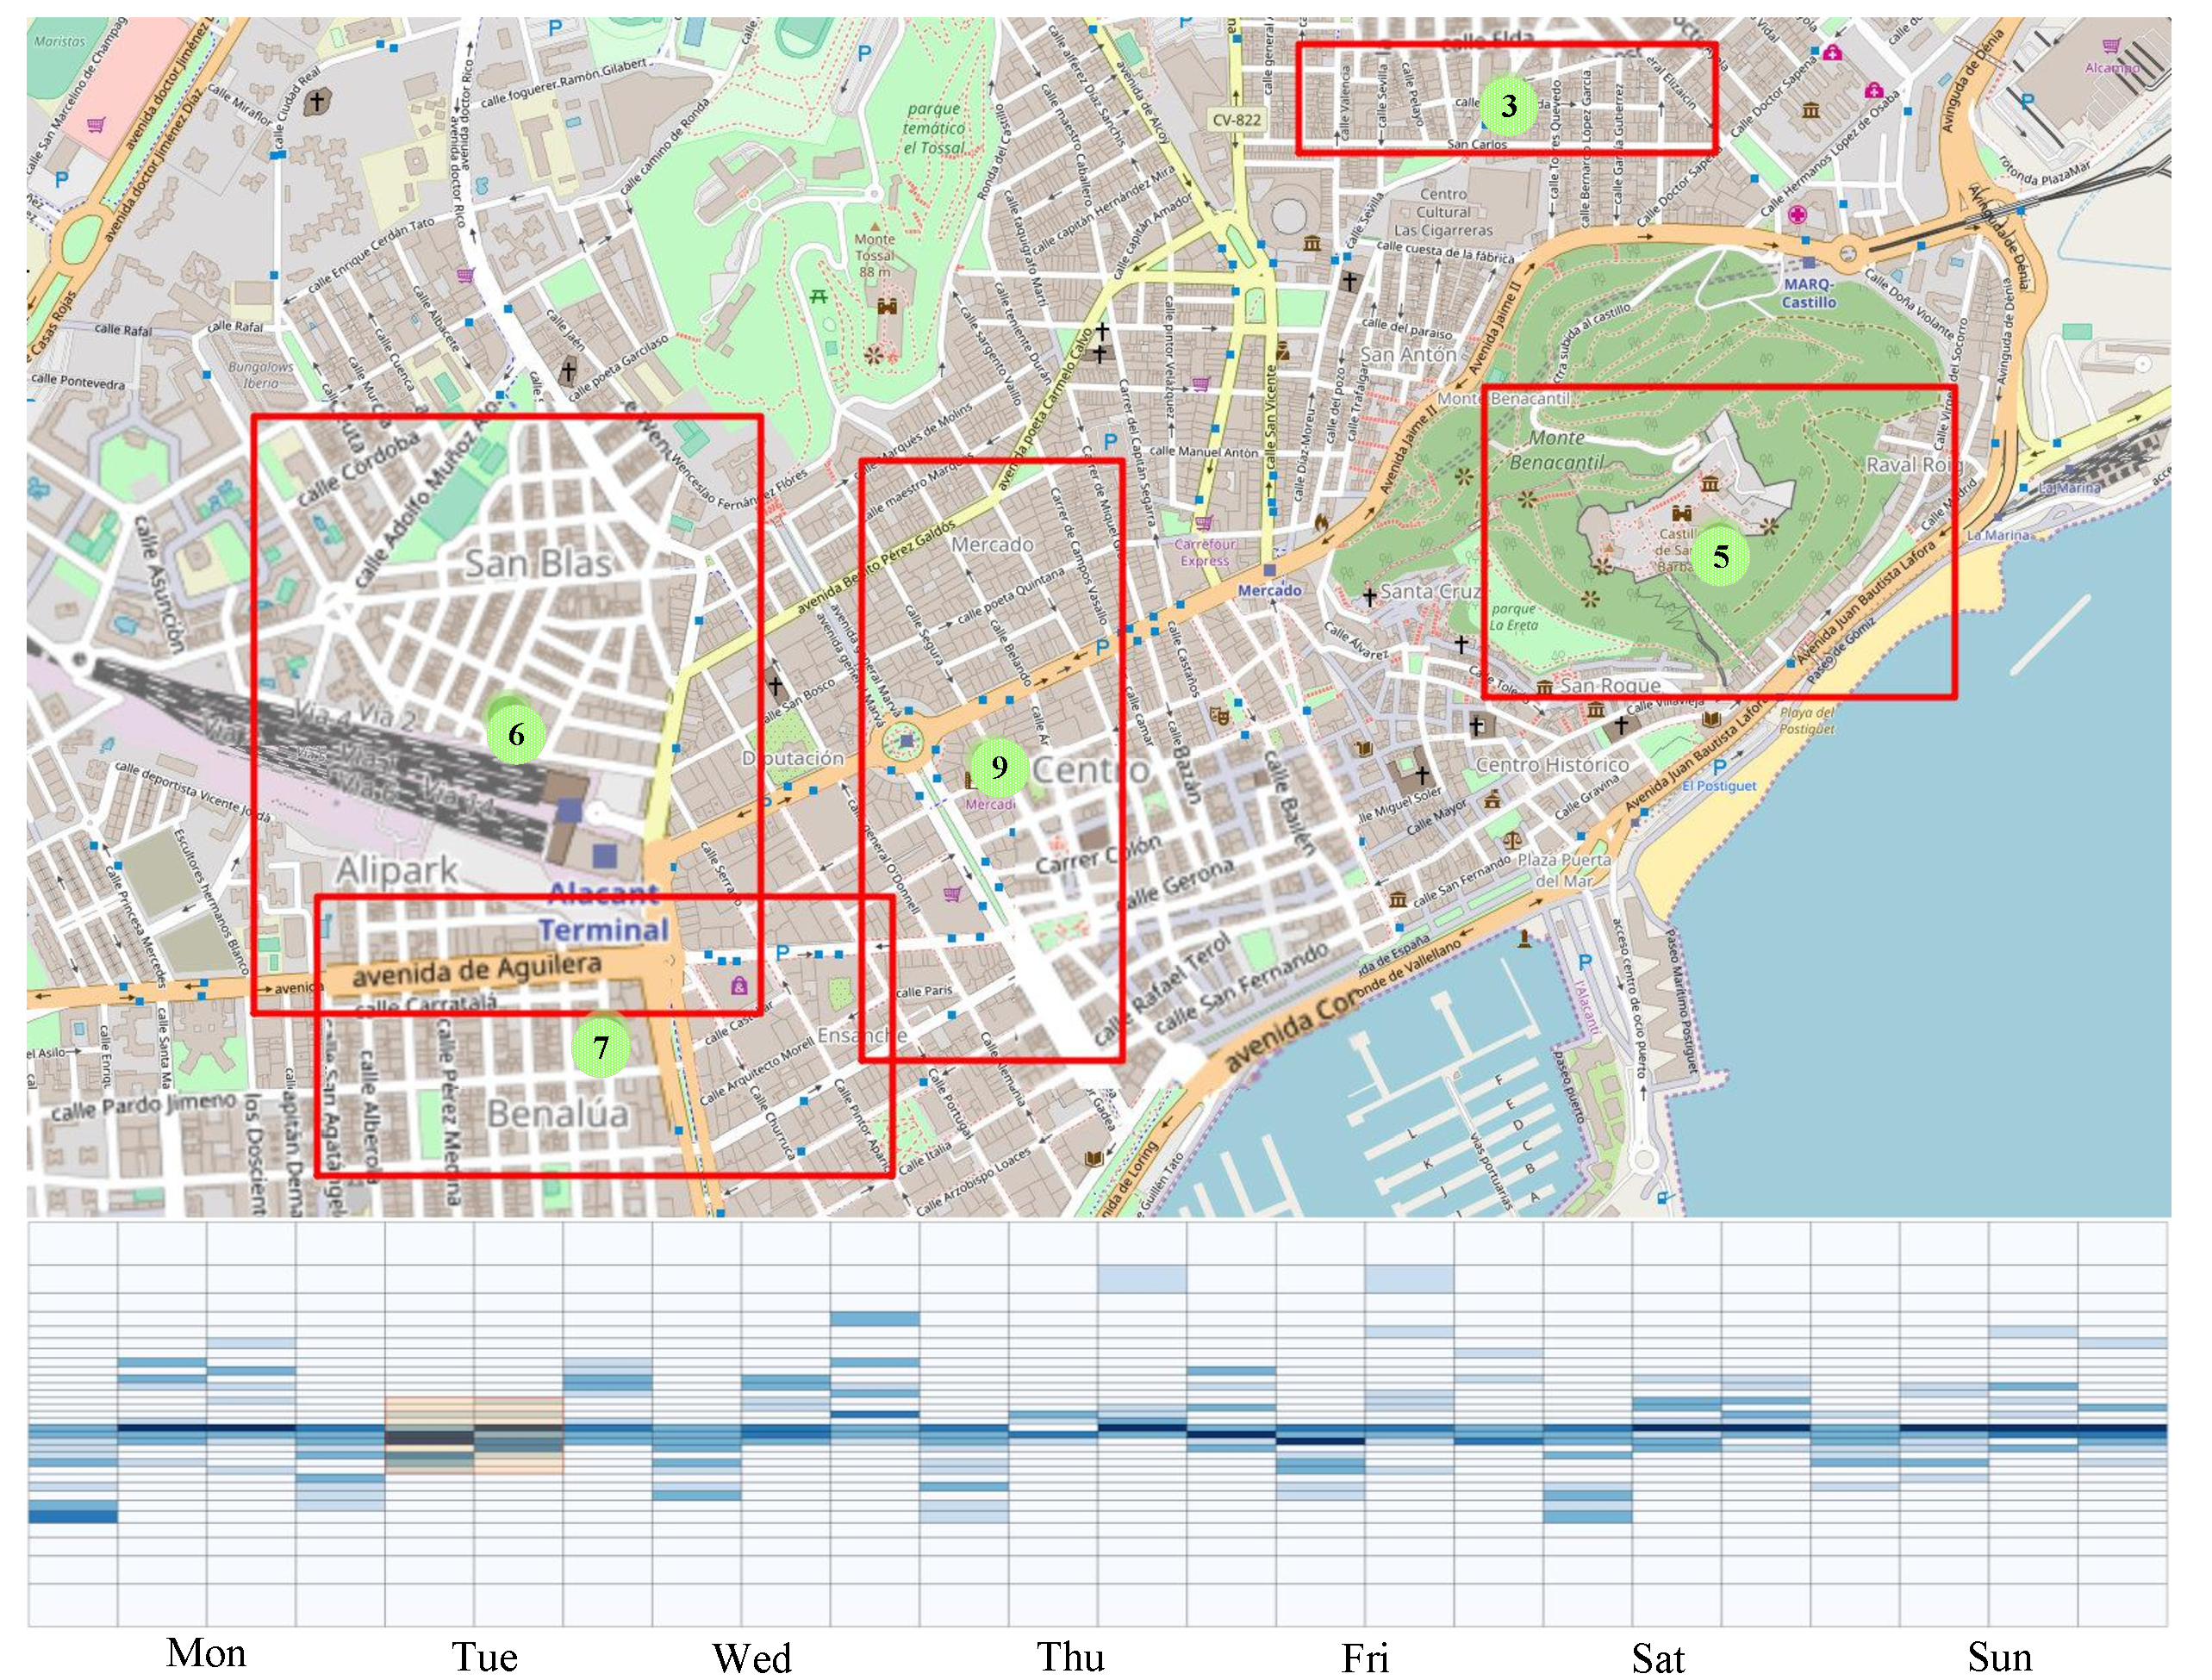
\includegraphics[width=\textwidth]{figures/timebox1.pdf}}
 \caption{Visualization of water consumption tile map summary in the city center of Alicante (map scale 1:5000).}
 \label{fig:alicante_example2}
\end{figure*}

\subsubsection{Map Visualizations}
\label{subsubsec:tilemap_sum_vis}
This visualization depicts a tile map summary of the geolocated time series that are contained within the currently visible part of the map. Whenever the user either moves around, zooms in and out the map, or draws a timebox on the time series domain, our summarization method is invoked to traverse the \hisax index and return the MBRs and tile map that correspond to the visible area. Once the results are returned, they are drawn on the map and time series frames respectively. Similarly to the bundle summary and in order to present the local density, the number of geolocated time series contained within each MBR is depicted using circles colored green for small numbers, yellow for larger and red for more densely populated MBRs. The time series frame is located on the bottom of the map and is essentially a depiction of the returned tile map, using lighter shades of blue for less populated tiles and darker shades for the more dense ones. The timeboxes are drawn on this frame, allowing a selection of arbitrary ranges on the value axis, while, on the time axis, the selection is forced to be aligned with the \isax segments.

An example of the tile map visualization is illustrated in Figure~\ref{fig:alicante_example2}, for the central area of Alicante, with $k=5$ MBRs, a SAX word length of $w=24$ and a maximum cardinality of $b=32$. An example timebox (depicted as an orange box) spans two \isax segments (corresponding to Tuesdays on the time axis) and has a range of one standard deviation on the value axis. The associated MBRs are depicted using red colored boxes. In this example, and within the chosen timebox, there exists a rather small amount of time series, indicating that not many households tend to maintain a lower water consumption behavior during Tuesdays.

\begin{figure*}[!ht]
 \centering
 \fbox{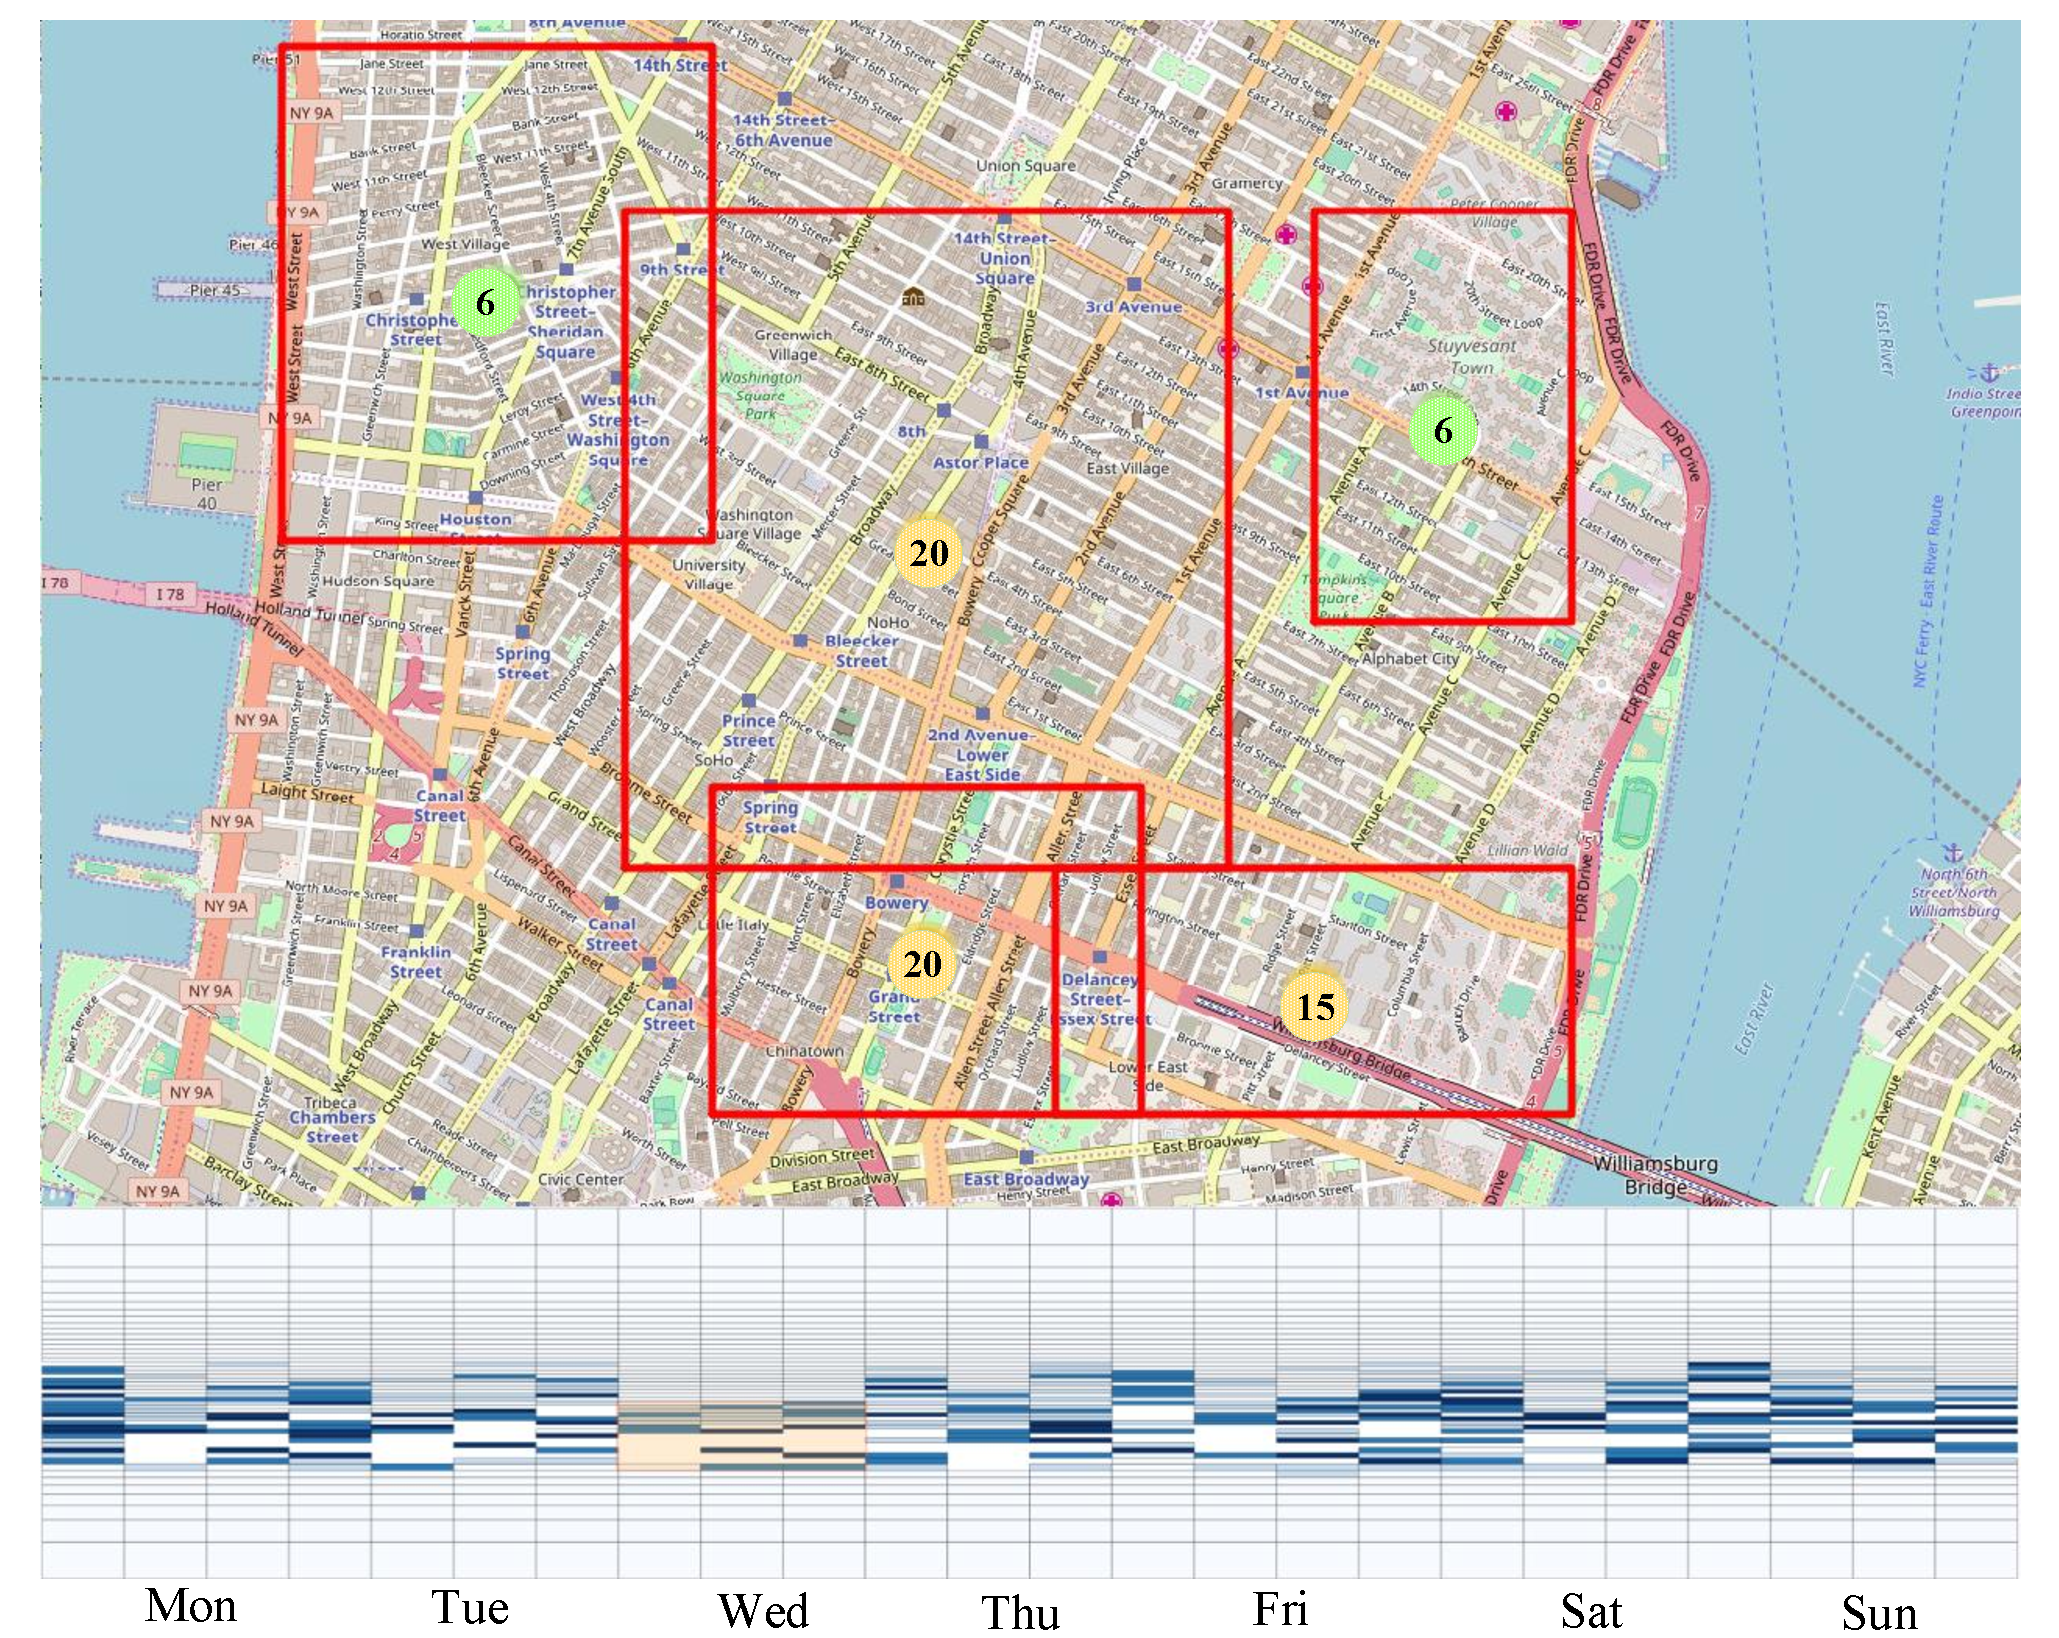
\includegraphics[width=\textwidth]{figures/timebox2.pdf}}
 \caption{Visualizing taxi dropoff tile map in Manhattan, NYC (map scale 1:10000).}
 \label{fig:nyc_example2}
\end{figure*}

Another example of the tile map visualization, depicting an area in Manhattan, New York is illustrated in Figure~\ref{fig:nyc_example2}, with $k=5$ MBRs, a SAX word length of $w=24$ and a maximum cardinality of $b=64$. This time, the timebox spans three \isax segments (representing Wednesdays) and a value range of one standard deviation. Since the selected range of taxi dropoffs is rather small, especially considering the fact that Manhattan is a busy area during the whole week, the depicted MBRs indicate that, during Wednesdays, there are quieter zones in these specific areas. Such information could be leveraged for searching a quieter neighborhood within the city.

\subsubsection{Performance Evaluation}
\label{subsubsec:tilemap_sum_benchmarking}

\paragraph{Parameters.} Similarly to the bundle summary, we performed preliminary tests against the synthetic dataset to fine-tune the parameters. We built the \hisax index setting the maximum number of entries per node to $M=200$, a maximum cardinality of $b=512$ and a default SAX word length of $w=8$. We have set the number of resulting MBRs to $k = 5$ for its leaf nodes. Table~\ref{tab:parameters2_vis} lists the range of values for the rest of the parameters.

\begin{table}[!ht]
\centering
\caption{Parameters in tests for tile map summaries}
\begin{footnotesize}
\begin{tabular}{lc} 
\hline
{\em Parameter} &{\em Values} \\
\hline
Timebox time range ($|p_t|$) & 1, {\bf 2}, 3, 4, 5 \\
Timebox value range ($|p_v|$) & 1$\sigma$, 1.5$\sigma$, {\bf 2$\sigma$}, 2.5$\sigma$, 3$\sigma$ \\
\hline
\end{tabular}
\end{footnotesize}
\label{tab:parameters2_vis}
\end{table}

\paragraph{Baseline method for detailed summaries.} Similarly to the bundle summary, we also compare with a more detailed baseline implementation in terms of accuracy and time required to fetch the results. The spatial part of the detailed summary is generated by performing $k$-means clustering on the filtered raw time series themselves and generating the resulting MBRs, instead of performing the clustering on each node's resulting MBRs. The tile map of the detailed summary has the exact same structure with the one of tile map summary. The difference among the two tile maps, since in the detailed summary the raw time series are used, lies in the way the count of each tile is augmented. Instead of increasing the count of the tiles where the SAX word's segments of a time series reside, we increase the count of the tiles where each time series point falls within.

\paragraph{Results.} We evaluate the performance of the tile map summary for different zoom levels and timebox sizes. For the comparison between the two tile maps we use the {\em root mean squared error} (RMSE) on the difference among the counts between each pair of corresponding tiles. As mentioned, the detailed tile map is generated using the raw time series. This essentially generates tile maps with larger counts, since instead of only incrementing the count once for a SAX word's segment of a time series, it may be incremented multiple times, as each word's segment is derived from $n/w$ time series points ($n$ is the length of time series and $w$ is the SAX word length). To compensate this, we divide the count of each tile of the detailed summary with $n/w$.

Conclusively, the root mean squared error among two tile maps is calculated as follows:

\begin{equation} \label{eq:rmse}
RMSE(tmap, tmap') = \sqrt{\frac{1}{w \times h}\displaystyle \sum_{i=1}^{w} \sum_{j=1}^{h}(c[i,j].cnt - \frac{c'[i,j].cnt}{n/w})^2} 
\end{equation}

\noindent where $tmap$ and $tmap'$ are respectively the tile maps from our method (Section~\ref{subsec:tilemapvis}) and the detailed summary, while $c[i,j].cnt$ and $c'[i,j].cnt$ are the corresponding counts of the $(i,j)$ tile in both summaries and $h$ is the number of y-axis breakpoints. For measuring the spatial accuracy, we follow the same rationale as in the evaluation of bundle summaries. Similarly, we evaluate the trade-off between responsiveness and accuracy of our approach. The detailed summary is expected to have a higher accuracy; however, since both spatial and time series summaries are calculated using the raw geolocated time series, we expect a trade-off in responsiveness, especially for larger datasets.

Figure~\ref{subfig:geo_iSAX_zoom} shows the traversal costs for different map scales for each of the three datasets. For the taxi and water datasets, the response time is almost instant due to their smaller sizes, ranging up to at most 100 milliseconds. For the case of the synthetic dataset and due to its high density, the response time is higher, starting from approximately 2.25 seconds for larger spatial areas of interest and falling down to 1.5 seconds as the map scale becomes larger (i.e., smaller areas). The rather higher response time for the tile map summary is due to the fact that in order to be calculated, the \hisax's leaf nodes have to be accessed to obtain the locations and maximum cardinality SAX words to generate the summary. However, it should be noted that this is a rather worst case scenario, since the synthetic dataset was generated to be very highly dense as a stress test. The response time is not dramatically reduced for larger map scales, since \hisax is a time series-first hybrid index and high overlapping of its MBRs is expected, so larger spatial areas of interest tend to intersect with the MBRs of many nodes, negatively impacting performance. As it is apparent, at a map scale of 1:500, the performance is more abruptly improved as the nodes of the index begin to be more aggressively pruned.

Similar results are also observed for different timebox sizes, as depicted in Figure~\ref{subfig:geo_iSAX_timeboxes}. The taxi and water datasets almost instantly generate the summaries along all timebox sizes. As a reminder, the timebox size is measured in terms of number of SAX segments selected in the time axis and standard deviation range selected in the value axis. In the figure, time range $|p_t|$ denotes the number of SAX segments, whereas value range $|p_v|$ expresses the standard deviation range selected for each timebox. For larger timebox sizes, the index traversal is slower as expected, as more nodes tend to satisfy the rather loose constraints. For the same reasons, the response time is improved up to around 1500 milliseconds as the timebox size gets smaller.

\begin{figure}[!t]
 \centering
 \subfloat[Response time for different map scales.]{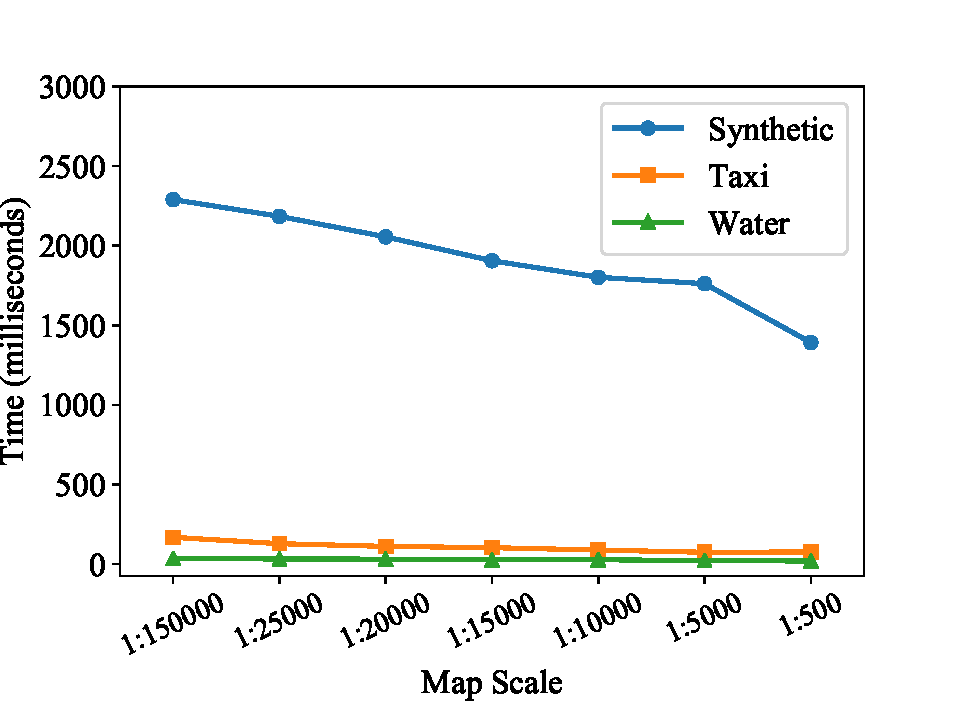
\includegraphics[width=0.45\textwidth]{figures/geo_iSAX_zoom.pdf}\label{subfig:geo_iSAX_zoom}}
 \subfloat[Response time for different timebox sizes.]{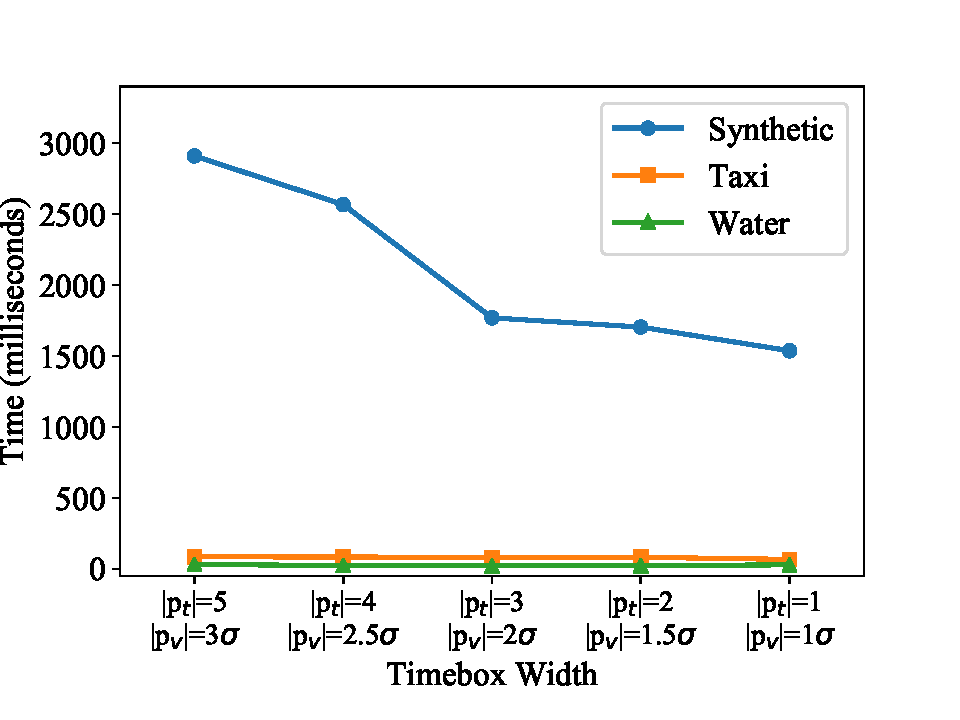
\includegraphics[width=0.45\textwidth]{figures/geo_iSAX_timeboxes.pdf}\label{subfig:geo_iSAX_timeboxes}}\
\caption{Response time for different map scales and timebox sizes.}
\label{fig:geo_iSAX_zoom_timebox}
\end{figure}

\begin{figure}[!t]
 \centering
 \subfloat[Accuracy in spatial domain.]{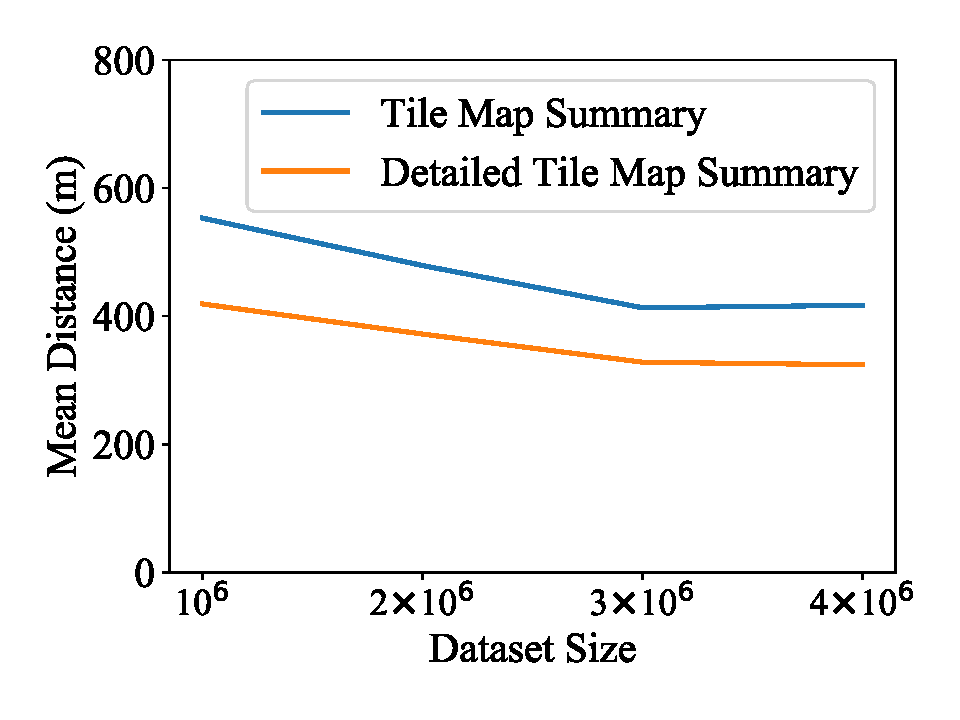
\includegraphics[width=0.30\textwidth]{figures/geo_iSAX_error_sp.pdf}\label{subfig:geo_iSAX_error_sp}}
 \subfloat[Accuracy in time series domain.]{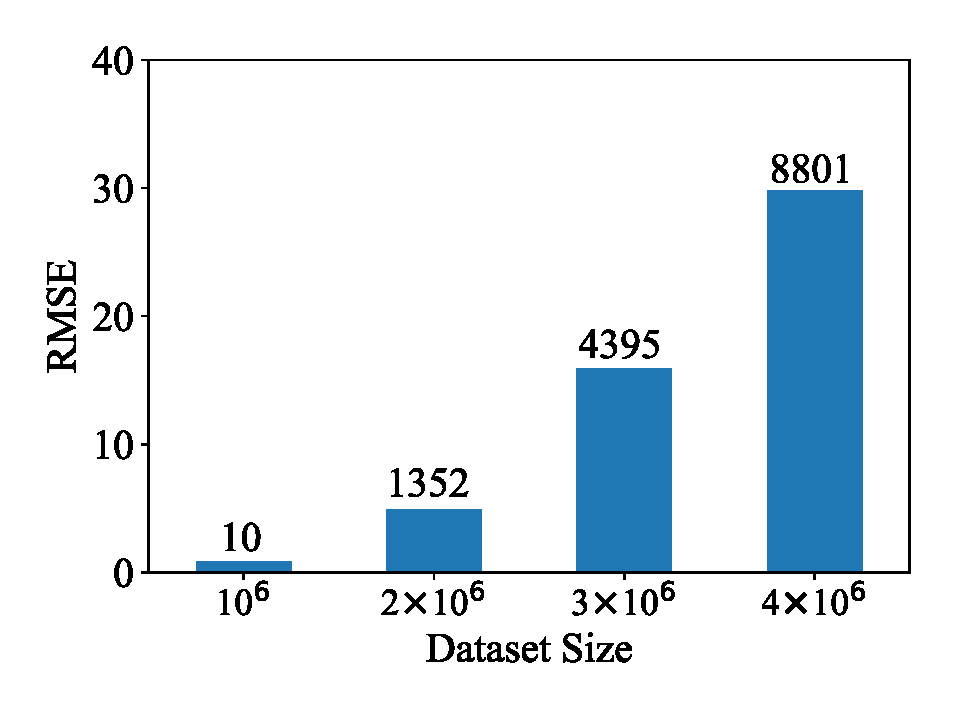
\includegraphics[width=0.30\textwidth]{figures/geo_iSAX_tilemapDiff.pdf}\label{subfig:geo_iSAX_tilemapDiff}}
 \subfloat[Response time.]{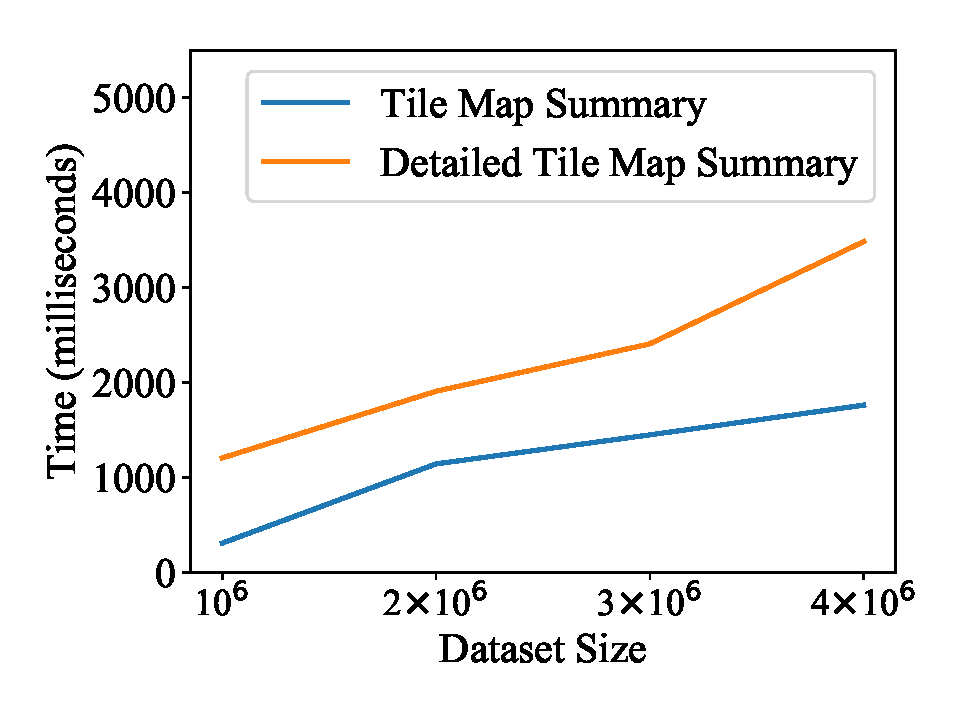
\includegraphics[width=0.30\textwidth]{figures/geo_iSAX_time.pdf}\label{subfig:geo_iSAX_time}}\
\caption{Assessment of tile map summarization.}
\label{fig:geo_iSAX_error}
\end{figure}

Figure~\ref{fig:geo_iSAX_error} demonstrates the  trade-off between accuracy and responsiveness by comparing the proposed tile map summary and its detailed implementation. As it can be easily observed, the difference between the spatial mean Euclidean distance among the raw data and their closest MBRs (Figure\ref{subfig:geo_iSAX_error_sp}) is between 150 and 200 meters for all dataset sizes. In both cases, it is rather larger for smaller datasets, slowly diminishing as their size gets larger, indicating an improvement of both summaries for larger data. It is worth noting that the difference from the baseline implementation also seems to be slightly reduced for larger datasets. Figure~\ref{subfig:geo_iSAX_tilemapDiff} illustrates the RMSE between the two tile maps using Equation~\ref{eq:dist_ts}. The number at the top of each bar is the count of results returned using the same constraints (spatial rectangle, timebox) over each dataset. It is apparent that the quality of the tile map summary worsens for a larger number of participating time series, increasingly diverging from the detailed version. Still, the loss in both spatial and tile map accuracy is compensated in terms of response time as depicted in Figure~\ref{subfig:geo_iSAX_time}. The detailed implementation requires up to twice the time to generate the summary for all dataset sizes, while its overhead compared to the tile map summary is increasing with larger datasets. Consequently, there is a clear trade-off between accuracy and response time in both domains, allowing an increase in responsiveness without much sacrifice in accuracy.
